%%%%%%%%%%%%%%%%%%%%%%%%%%%%%%%%%%%%%%%%%%%%%%%%%%%%%%%%%%%%%%%%%%%%%%%%%%%%%%%%
%Tutorial slides on Python.
%
% Author: FOSSEE 
% Copyright (c) 2009, FOSSEE, IIT Bombay
%%%%%%%%%%%%%%%%%%%%%%%%%%%%%%%%%%%%%%%%%%%%%%%%%%%%%%%%%%%%%%%%%%%%%%%%%%%%%%%%

\documentclass[14pt,compress]{beamer}
%\documentclass[draft]{beamer}
%\documentclass[compress,handout]{beamer}
%\usepackage{pgfpages} 
%\pgfpagesuselayout{2 on 1}[a4paper,border shrink=5mm]

% Modified from: generic-ornate-15min-45min.de.tex
\mode<presentation>
{
  \usetheme{Warsaw}
  \useoutertheme{infolines}
  \setbeamercovered{transparent}
}

\usepackage[english]{babel}
\usepackage[latin1]{inputenc}
%\usepackage{times}
\usepackage[T1]{fontenc}

% Taken from Fernando's slides.
\usepackage{ae,aecompl}
\usepackage{mathpazo,courier,euler}
\usepackage[scaled=.95]{helvet}

\definecolor{darkgreen}{rgb}{0,0.5,0}

\usepackage{listings}
\lstset{language=Python,
    basicstyle=\ttfamily\bfseries,
    commentstyle=\color{red}\itshape,
  stringstyle=\color{darkgreen},
  showstringspaces=false,
  keywordstyle=\color{blue}\bfseries}

%%%%%%%%%%%%%%%%%%%%%%%%%%%%%%%%%%%%%%%%%%%%%%%%%%%%%%%%%%%%%%%%%%%%%%
% Macros
\setbeamercolor{emphbar}{bg=blue!20, fg=black}
\newcommand{\emphbar}[1]
{\begin{beamercolorbox}[rounded=true]{emphbar} 
      {#1}
 \end{beamercolorbox}
}
\newcounter{time}
\setcounter{time}{0}
\newcommand{\inctime}[1]{\addtocounter{time}{#1}{\tiny \thetime\ m}}

\newcommand{\typ}[1]{\lstinline{#1}}

\newcommand{\kwrd}[1]{ \texttt{\textbf{\color{blue}{#1}}}  }

%%% This is from Fernando's setup.
% \usepackage{color}
% \definecolor{orange}{cmyk}{0,0.4,0.8,0.2}
% % Use and configure listings package for nicely formatted code
% \usepackage{listings}
% \lstset{
%    language=Python,
%    basicstyle=\small\ttfamily,
%    commentstyle=\ttfamily\color{blue},
%    stringstyle=\ttfamily\color{orange},
%    showstringspaces=false,
%    breaklines=true,
%    postbreak = \space\dots
% }

%%%%%%%%%%%%%%%%%%%%%%%%%%%%%%%%%%%%%%%%%%%%%%%%%%%%%%%%%%%%%%%%%%%%%%
% Title page
\title[Interactive Plotting]{Python for Science and Engg: Interactive Plotting}

\author[FOSSEE] {FOSSEE}

\institute[IIT Bombay] {Department of Aerospace Engineering\\IIT Bombay}
\date[] {11 January, 2010\\Day 1, Session 1}
%%%%%%%%%%%%%%%%%%%%%%%%%%%%%%%%%%%%%%%%%%%%%%%%%%%%%%%%%%%%%%%%%%%%%%

%\pgfdeclareimage[height=0.75cm]{iitmlogo}{iitmlogo}
%\logo{\pgfuseimage{iitmlogo}}


%% Delete this, if you do not want the table of contents to pop up at
%% the beginning of each subsection:
\AtBeginSubsection[]
{
  \begin{frame}<beamer>
    \frametitle{Outline}
    \tableofcontents[currentsection,currentsubsection]
  \end{frame}
}

\AtBeginSection[]
{
  \begin{frame}<beamer>
    \frametitle{Outline}
    \tableofcontents[currentsection,currentsubsection]
  \end{frame}
}

% If you wish to uncover everything in a step-wise fashion, uncomment
% the following command: 
%\beamerdefaultoverlayspecification{<+->}

%%\includeonlyframes{current,current1,current2,current3,current4,current5,current6}

%%%%%%%%%%%%%%%%%%%%%%%%%%%%%%%%%%%%%%%%%%%%%%%%%%%%%%%%%%%%%%%%%%%%%%
% DOCUMENT STARTS
\begin{document}

\begin{frame}
  \maketitle
\end{frame}

%% \begin{frame}
%%   \frametitle{Outline}
%%   \tableofcontents
%%   % You might wish to add the option [pausesections]
%% \end{frame}

\begin{frame}
  \frametitle{Workshop Schedule: Day 1}
  \begin{description}
	\item[Session 1] Mon 09:00--10:00
	\item[Session 2] Mon 10:05--11:05
	\item[Session 3] Mon 11:20--12:20
	\item[Session 4] Mon 12:25--13:25
        \item[Quiz 1] Mon 14:25--14:40
        \item[Exercises] Mon 14:40--15:25
        \item[Session 5] Mon 15:40--16:40
        \item[Quiz 2] Mon 16:45--17:00
  \end{description}
\end{frame}

\begin{frame}
  \frametitle{Workshop Schedule: Day 2}
  \begin{description}
	\item[Session 1] Tue 09:00--10:00
	\item[Session 2] Tue 10:05--11:05
	\item[Session 3] Tue 11:20--12:20
	\item[Session 4] Tue 12:25--13:25
        \item[Quiz 1]  Tue 14:25--14:40
        \item[Exercises] Tue 14:40--15:25
        \item[Session 5] Tue 15:40--16:40
        \item[Quiz 2]  Tue 16:45--17:00
  \end{description}
\end{frame}

\begin{frame}
  \frametitle{About the Workshop}
  \begin{block}{Intended Audience}
  \begin{itemize}
       \item Engg., Mathematics and Science teachers.
       \item Interested students from similar streams.
  \end{itemize}
  \end{block}  

  \begin{block}{Goal: Successful participants will be able to}
    \begin{itemize}
      \item Use Python as plotting, computational tool.
      \item Understand how to use Python as a scripting and problem solving language.
      \item Train students for the same.
    \end{itemize}
  \end{block}
\end{frame}

\section{Getting started}
\begin{frame}
\frametitle{Checklist}
  \begin{enumerate}
    \item IPython
    \item Editor: We recommend \alert{scite}.
    \item Data files: 
      \begin{itemize}
      \item \typ{sslc1.txt}
      \item \typ{pendulum.txt}
      \item \typ{points.txt}
      \item \typ{pos.txt}
      \item \typ{holmes.txt}
      \end{itemize}
    \item Python scripts: 
      \begin{itemize}
      \item \typ{sslc_allreg.py}
      \item \typ{sslc_science.py}
      \end{itemize}
    \item Images
      \begin{itemize}
      \item \typ{lena.png}
      \item \typ{smoothing.gif}
      \end{itemize}
  \end{enumerate}
\end{frame}

\begin{frame}[fragile]
\frametitle{Starting up \ldots}
\begin{block}{}
\begin{lstlisting}
  $ ipython -pylab  
\end{lstlisting} %$
\end{block}
\begin{lstlisting}     
  In []: print "Hello, World!"
  Hello, World!
\end{lstlisting}
Exiting
\begin{lstlisting}     
  In []: ^D(Ctrl-D)
  Do you really want to exit([y]/n)? y
\end{lstlisting}
\end{frame}

%% \begin{frame}[fragile]
%% \frametitle{Loops}
%% Breaking out of loops
%% \begin{lstlisting}     
%%   In []: while True:
%%     ...:     print "Hello, World!"
%%     ...:     
%%   Hello, World!
%%   Hello, World!^C(Ctrl-C)
%%   ------------------------------------
%%   KeyboardInterrupt                   

%% \end{lstlisting}
%% \end{frame}

\section{Plotting}

\subsection{Drawing plots}
\begin{frame}[fragile]
\frametitle{First Plot}
\begin{columns}
    \column{0.25\textwidth}
    \hspace*{-0.5in}
  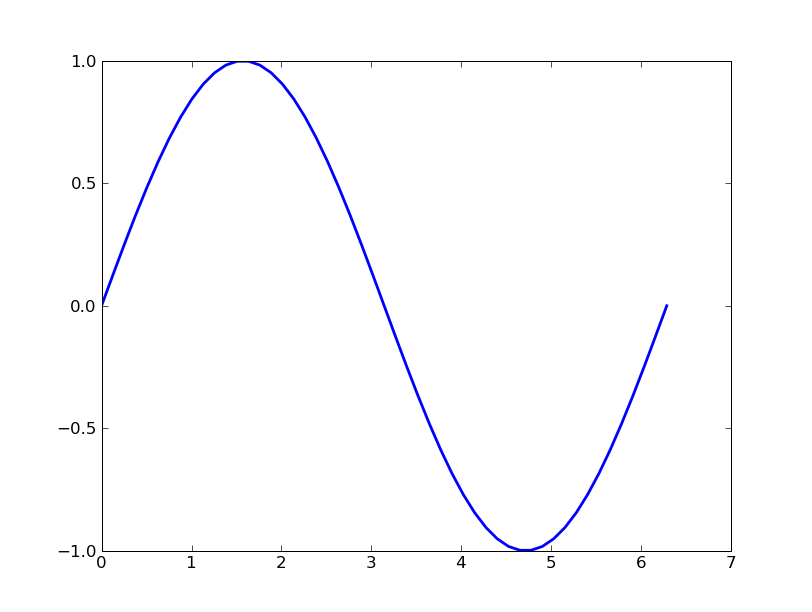
\includegraphics[height=2in, interpolate=true]{data/firstplot}
    \column{0.8\textwidth}
    \begin{block}{}
    \begin{small}
\begin{lstlisting}
In []: x = linspace(0, 2*pi, 50)
In []: plot(x, sin(x))
\end{lstlisting}
    \end{small}
    \end{block}
\end{columns}
\end{frame}


\begin{frame}[fragile]
\frametitle{Walkthrough}
\begin{block}{\typ{x = linspace(start, stop, num)} }
returns \typ{num} evenly spaced points, in the interval [\typ{start}, \typ{stop}].
\end{block}
\begin{lstlisting}
x[0] = start
x[num - 1] = end
\end{lstlisting}
\vspace*{.35in}
\begin{block}{\typ{plot(x, y)}}
plots \typ{x} and \typ{y} using default line style and color
\end{block}
%\inctime{10}
\end{frame}

\subsection{Decoration}
\begin{frame}[fragile]
\frametitle{Adding Labels}
\begin{columns}
  \column{0.25\textwidth}
  \hspace*{-0.45in}
  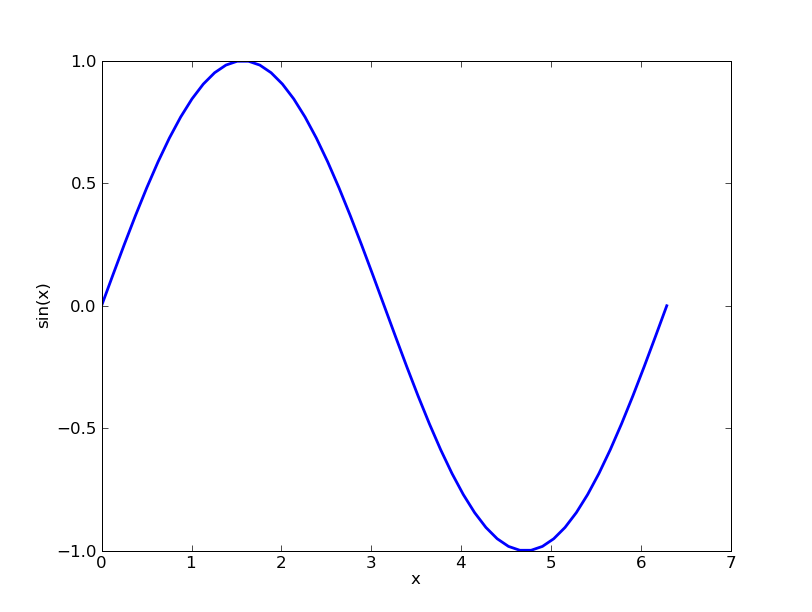
\includegraphics[height=2in, interpolate=true]{data/label}  
  \hspace*{0.5in}
  \column{0.55\textwidth}
  \begin{block}{}
  \small
  \begin{lstlisting}
In []: xlabel('x')

In []: ylabel('sin(x)')
  \end{lstlisting}
  \small
%  \end{lstlisting}
%\typ{xlabel(s)} sets the label of the \typ{x}-axis to \typ{s}

%  \begin{lstlisting}
  \end{block}
%\typ{ylabel(s)} sets the label of the \typ{y}-axis to \typ{s}
\end{columns}
\end{frame}

\begin{frame}[fragile]
\frametitle{Another example}
  \begin{lstlisting}
In []: clf()
  \end{lstlisting}
\emphbar{Clears the plot area.}
  \begin{lstlisting}
In []: y = linspace(0, 2*pi, 50)
In []: plot(y, sin(2*y))
In []: xlabel('y')
In []: ylabel('sin(2y)')
  \end{lstlisting}
\end{frame}

\subsection{More decoration}
\begin{frame}[fragile]
\frametitle{Title and Legends}
\vspace*{-0.15in}
%  \begin{block}{}
%  \small
\begin{lstlisting}
In []: title('Sinusoids')
In []: legend(['sin(2y)'])
\end{lstlisting}
%  \small
%  \end{block}
  \vspace*{-0.1in}
  \begin{center}
  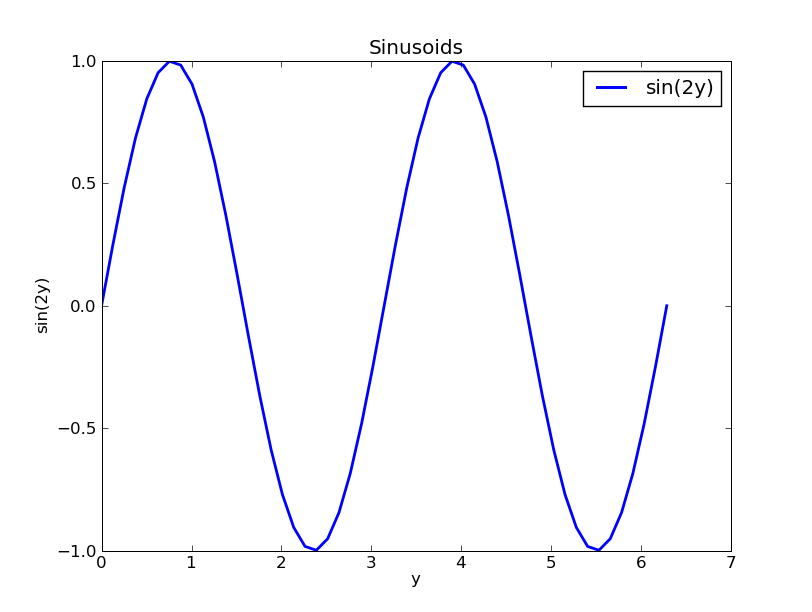
\includegraphics[height=2in, interpolate=true]{data/legend}  
  \end{center}
\end{frame}

\begin{frame}[fragile]
\frametitle{Legend Placement}
\begin{block}{}
    \small
\begin{lstlisting}
In []: legend(['sin(2y)'], loc = 'center')
\end{lstlisting}
\end{block}

\begin{columns}
    \column{0.6\textwidth}
 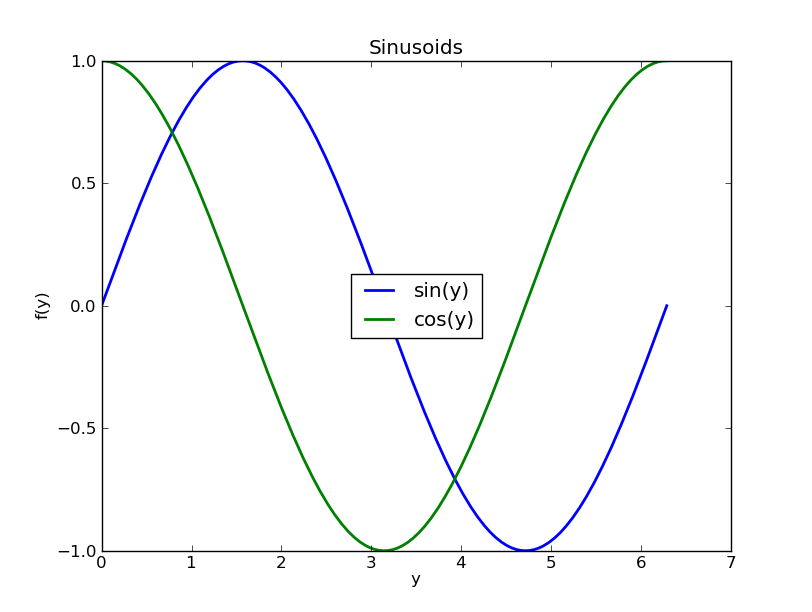
\includegraphics[height=2in, interpolate=true]{data/position}  
\column{0.45\textwidth}
\vspace{-0.2in}
\begin{lstlisting}
'best' 
'right'
'center'
\end{lstlisting}
\end{columns}
\end{frame}

%% \begin{frame}[fragile]
%%   \frametitle{For arbitrary location}
%% \vspace*{-0.1in}
%% \begin{lstlisting}
%% In []: legend(['sin(2y)'], loc=(.8,.1)) 
%% \end{lstlisting}
%% \emphbar{Specify south-east corner position}
%% %\vspace*{-0.2in}
%% \begin{center}
%%   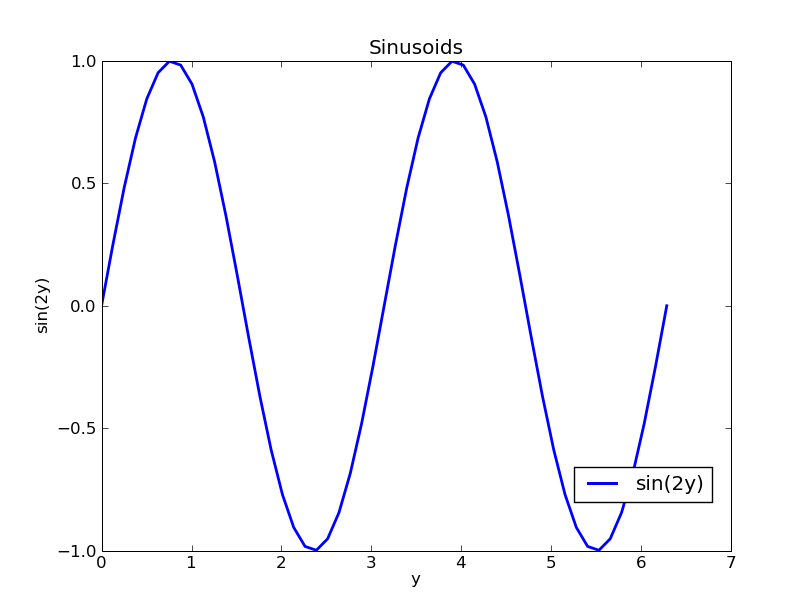
\includegraphics[height=2in, interpolate=true]{data/loc}  
%% \end{center}
%% %\inctime{10}
%% \end{frame}

\begin{frame}[fragile]
\frametitle{Saving \& Closing}
\begin{lstlisting}
In []: savefig('sin.png')

In []: close()
\end{lstlisting}
\end{frame}

\section{Multiple plots}
\begin{frame}[fragile]
\frametitle{Overlaid Plots}
\begin{lstlisting}
In []: clf()
In []: plot(y, sin(y))
In []: plot(y, cos(y))
In []: xlabel('y')
In []: ylabel('f(y)')
In []: legend(['sin(y)', 'cos(y)']) 
\end{lstlisting}
\emphbar{By default plots would be overlaid!}
\end{frame}

\begin{frame}[fragile]
\frametitle{Plotting separate figures}
\begin{lstlisting}
In []: clf()
In []: figure(1)
In []: plot(y, sin(y))
In []: figure(2)
In []: plot(y, cos(y))
In []: figure(1)
In []: title('sin(y)')
In []: close()
In []: close()
\end{lstlisting}
\end{frame}

\begin{frame}[fragile]
\frametitle{Showing it better}
\vspace{-0.15in}
\begin{lstlisting}
In []: plot(y, sin(y), 'g')

In []: clf()
In []: plot(y, cos(y), 'r', linewidth=2)
\end{lstlisting}
\vspace*{-0.2in}
\begin{center}
  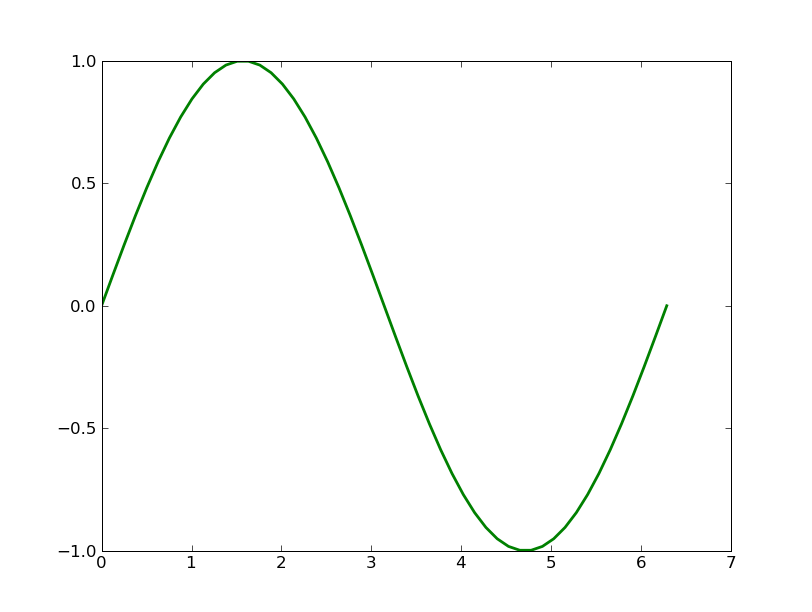
\includegraphics[height=2.2in, interpolate=true]{data/green}  
\end{center}
%\inctime{10}
\end{frame}

\begin{frame}[fragile]
\frametitle{Annotating}
\vspace*{-0.15in}
\begin{lstlisting}
In []: annotate('local max', xy=(1.5, 1))
\end{lstlisting}
\vspace*{-0.2in}
\begin{center}
  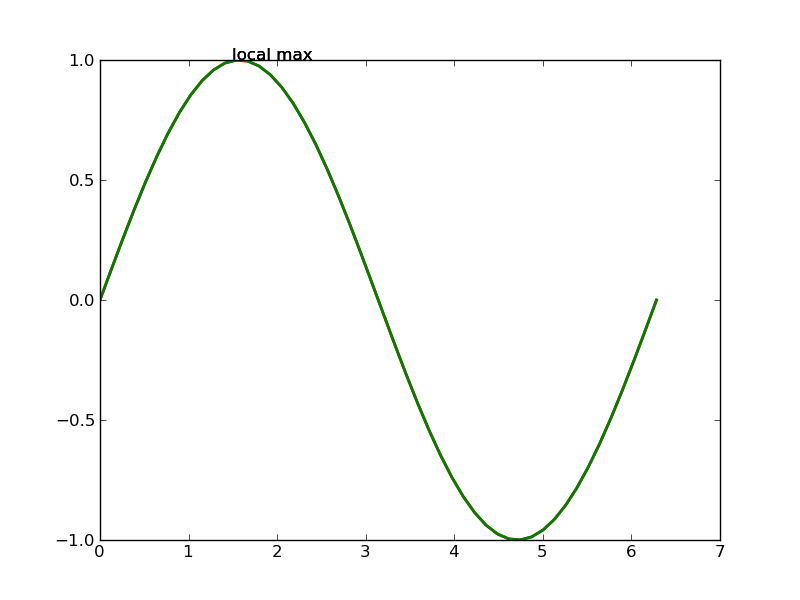
\includegraphics[height=2in, interpolate=true]{data/annotate}  
\end{center}
\end{frame}

\begin{frame}[fragile]
\frametitle{Axes lengths}
\emphbar{Get the axes limits}
  \begin{lstlisting}
In []: xmin, xmax = xlim() 
In []: ymin, ymax = ylim() 
  \end{lstlisting}
\emphbar{Set the axes limits}
  \begin{lstlisting}
In []: xmax = 2*pi
In []: xlim(xmin, xmax) 
In []: ylim(ymin-0.2, ymax+0.2) 
  \end{lstlisting}
\end{frame}

\begin{frame}[fragile]
\frametitle{Review Problem}
\begin{enumerate}
\item Plot x, -x, sin(x), xsin(x) in range $-5\pi$ to $5\pi$
\item Add a legend
\item Annotate the origin
\item Set axes limits to the range of x
\end{enumerate}
\vspace*{-0.1in}
\begin{center}
  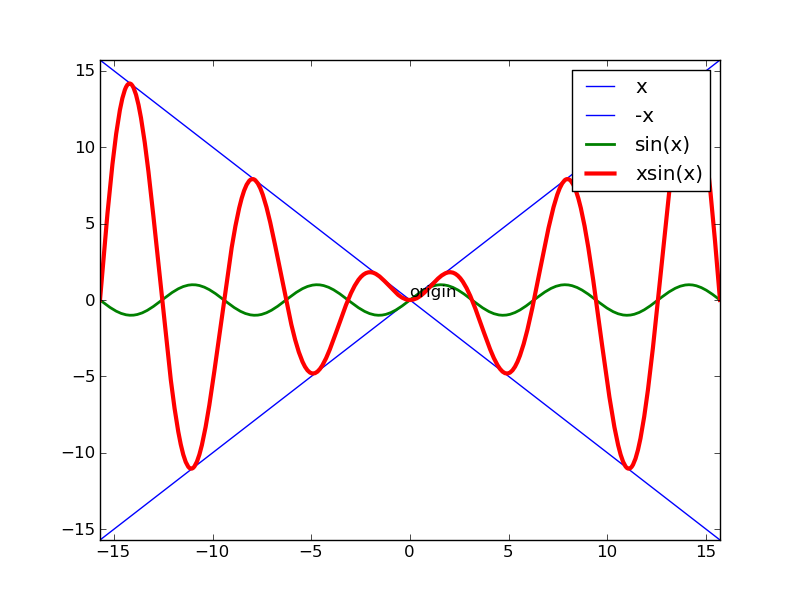
\includegraphics[height=2.1in, interpolate=true]{data/four_plot}  
\end{center}
\end{frame}

\begin{frame}[fragile]
\frametitle{Review Problem \ldots}
\alert{Plotting \ldots}
\begin{lstlisting}
In []: x=linspace(-5*pi, 5*pi, 500)
In []: plot(x, x, 'b')
In []: plot(x, -x, 'b')
In []: plot(x, sin(x), 'g', linewidth=2)
In []: plot(x, x*sin(x), 'r', 
            linewidth=3)
\end{lstlisting}
$\vdots$
\end{frame}

\begin{frame}[fragile]
\frametitle{Review Problem \ldots}
\alert{Legend \& Annotation\ldots}
\begin{lstlisting}
In []: legend(['x', '-x', 'sin(x)', 
               'xsin(x)'])
In []: annotate('origin', xy = (0, 0))
\end{lstlisting}
\alert{Setting Axes limits\ldots}
\begin{lstlisting}
In []: xlim(-5*pi, 5*pi)
In []: ylim(-5*pi, 5*pi)
\end{lstlisting}
\end{frame}

\begin{frame}[fragile]
\frametitle{Saving Commands}
Save commands of review problem into file
\begin{itemize}
\item Use \typ{\%hist} command of IPython 
\item Identify the required line numbers
\item Then, use \typ{\%save} command of IPython
\end{itemize}
\typ{In []: \%hist}\\
\typ{In []: \%save four_plot.py} \alert{\typ{16 18-27}} 
\begin{block}{Careful about errors!}
  \kwrd{\%hist} will contain the errors as well,\\
  so be careful while selecting line numbers.
\end{block}
\end{frame}

\begin{frame}
\frametitle{Python Scripts\ldots}
 This is called a Python Script.
 \begin{itemize}
 \item run the script in IPython using \typ{\%run -i four_plot.py}\\
 \end{itemize}
\end{frame}

\begin{frame}[fragile]
  \frametitle{What did we learn?}
  \begin{itemize}
    \item \kwrd{\%hist}
    \item Saving commands to a script
    \item Running a script using \kwrd{\%run -i}
    \item Creating simple plots.
    \item Adding labels and legends.
    \item Annotating plots.
    \item Changing the looks: size, linewidth
  \end{itemize}
\end{frame}

\end{document}

%% Questions for Quiz %%
%% ------------------ %%

\begin{frame}[fragile]
\frametitle{\incqno }
Draw (roughly) the plot obtained by the following:
\begin{lstlisting}
In []: x = linspace(0, 2*pi, 3)
In []: plot(x, sin(x))
\end{lstlisting}
\end{frame}

\begin{frame}[fragile]
\frametitle{\incqno }
Describe the plot produced by the following:
\begin{lstlisting}
In []: x = linspace(0, 2*pi, 50)
In []: plot(x, cos(x), 'go')
\end{lstlisting}
\end{frame}

\begin{frame}
\frametitle{\incqno }
How will you plot the previous graph with line width set to 3?  How will
you set the $x$ and $y$ labels of the plot?
\end{frame}

\begin{frame}
\frametitle{\incqno }
How will you set the x and y axis limits so that the region of interest
is in the rectangle $(0, -1.5)$ (left bottom coordinate) and $(2\pi,
1.5)$ (right top coordinate)?
\end{frame}

\begin{frame}
\frametitle{\incqno }
What ipython magic command do you use to obtain the lines of code you have already typed in the interpreter? What command do you use to save them?
\end{frame}

\begin{frame}
\frametitle{\incqno }
The following code snippet has an error/bug:
\begin{lstlisting}
In []: y = linspace(0, 2*pi, 50)
In []: plot(y, sin(y))
In []: clf()
In []: plot(y, cos(y))
In []: legend(['sin(y)', 'cos(y)']) 
\end{lstlisting}
What is the error? How do you fix it?  
\end{frame}
